\chapter{Rivelatori a semiconduttore}
L'utilizzo di camere a ionizzazione a stato solido con semiconduttori pu\`o semplificare notevolmente la struttura di un rivelatore:
l'elevata densit\`a di portatori di carica permette, infatti, di ottenere rivelatori di dimensioni ridotte (sono sufficienti 300 $\mu$m di Si), inoltre,
grazie alla bassa energia di ionizzazione e alla presenza di portatori di carica positivi e negativi, \`e possibile ottenere segnali sufficientemente
ampii senza ricorrere alla moltiplicazione.
Per utilizzare questi rivelatori \`e necessario che le cariche abbiano una vita media elevata e che la loro mobilit\`a sia sufficiente, pur mantenendo
una corrente di buio ridotta.
Queste caratteristiche sono presenti nel silicio, germanio e GaAs, sebbene i primi due a temperatura ambiente abbiano una corrente di buio troppo elevata.
\section{Semiconduttori intrinseci}
In un semiconduttore intrinseco il numero di portatori di carica in banda di conduzione pu\`o essere determinato attraverso:
\begin{equation*}
n^2 = N_c N_v e^{\frac{E_g}{k_B T}}
\end{equation*}
con $N_c$ numero di stati ai margini della banda di conduzione e $N_v$ in banda di valenza.
Posto $n$ il numero di portatori di carica negativi e $p$ numero di quelli positivi (lacune) vale
che $n=p$ e che $np=n^2$.
In un silicio a temperatura ambiente $n_i \sim 10^{10}$ e in un germanio $\sim 10^{13}$.\\
Per quanto riguarda la resistivit\`a di questi materiali, la velocit\`a delle cariche \`e data dalla relazione:
\begin{equation*}
v = \mu_{e,h} \, E
\end{equation*}
La mobilit\`a delle lacune \`e inferiore, ma dello stesso ordine di grandezza, rispetto a quella degli elettroni;
in generale la resistivit\`a pu\`o essere definita come:
\begin{equation*}
\rho = \frac{1}{q(\mu_n n + \mu_h p)}
\end{equation*}
Nel Si o Ge intrinseco, il numero di portatori di carica liberi per agitazione termica \`e troppo pi\`u grande rispetto a quelli prodotti
dalla ionizzazione, per questo non sono utilizzabili nella forma pura ed \`e necessario ricorrere alle giunzioni di materiali drogati.
\section{Semiconduttori estrinseci o drogati}
Introducendo delle impurezze nel cristallo semiconduttore si effettua l'operazione di drogaggio; mediante il drogaggio del materiale si riescono ad ottenere conducibilit\`a maggiori.
Esistono due tipi di drogaggio:
\begin{itemize}
\item tipo p, si introduce un materiale con un elettrone di valenza in meno e si introduce uno stato intermedio spostato verso la banda di valenza;
in questo modo si favorisce la presenza di lacune nel materiale
\item tipo n, si introduce un materiale con un elettrone di valenza in pi\`u e si introduce uno stato intermedio spostato verso la banda di conduzione;
in questo modo si favorisce l'elettrone eccedente ad entrare nella banda di conduzione
\end{itemize}
Introducendo le impurezze, le energie di ionizzazione vanno nei meV, rendendo il materiale un buon conduttore a temperatura ambiente.\
Chiamando $N_D$ il numero di donori (impurezze tipo n) e $N_A$ il numero di accettori (tipo p) se esse sono numerose si pu\`o affermare
che $n \approx N_D$ (in un tipo n) oppure $p \approx N_A$ (in un tipo p).
Inoltre il numero di portatori di carica di segno opposto potr\`a essere calcolato come:
\begin{equation*}
p \;(n) = \frac{n_i^2}{n \; (p)} \approx \frac{n_i^2}{N_D\;(N_A)}
\end{equation*}
In queste condizioni di drogaggio si parla di \textbf{semiconduttori estrinseci};
se $N_A \asymp N_D$ si parla di materiali compensati, se $N_{A,D} \ge 10^{19} - 10^{20}$ cm$^{-3}$ si parla di materiali pesantemente drogati
in quanto si \`e raggiunto il livello di conducibilit\`a dei metalli.
\section{Rivelatori basati su i semiconduttori}
\`E possibile immaginare un rivelatore che si occupi di raccogliere le coppie elettrone-lacuna prodotte in un cristallo semiconduttore in seguito
alla ionizzazione prodotta da una particella.
In un semiconduttore l'energia media per produrre una coppia lacuna-elettrone \`e nell'ordine dei 3 eV (simile al gap di energia tra le bande),
circa 10 volte inferiore a quello nei gas: questo si ripercuote sulla risoluzione, che migliora notevolmente.
Una stima brutale del miglioramento pu\`o essere fatta in approssimazione di risoluzione poissoniana:
poich\`e, a parit\`a di energia, in un semiconduttore si producono 10 volte pi\`u cariche rispetto ad un gas, allora il rapporto tra le risoluzioni
percentuali ($\propto \frac{1}{\sqrt{N}}$) vale:
\begin{equation*}
\frac{R_{SEMI}}{R_{GAS}} = \frac{\sqrt{N}}{\sqrt{10 N}} \approx \frac{1}{3}
\end{equation*}
per cui la risoluzione migliora di un fattore $\frac{1}{3}$. 
In realt\`a, il miglioramento \`e ancora maggiore per via del fattore di Fano.\\
La configurazione pi\`u semplice attuabile porterebbe a introdurre del silicio puro tra due elettrodi, ma purtroppo l'elevata conducibilit\`a
del silicio porta ad avere correnti di buio troppo grandi rispetto alle correnti prodotte dagli eventi;
per questo motivo \`e necessario ricorrere alle giunzioni tra materiali drogati.
\section{La giunzione p-n}
Consideriamo due semiconduttori drogati uno di tipo p e uno di tipo n.
Da un lato si ha una sovrabbondanza di lacune, dall'altra una sovrabbondanza di elettroni;
quando i due semiconduttori vengono messi a contatto, si forma una corrente detta di diffusione dovuta alla ricombinazione delle lacune con gli elettroni.
Lungo la giunzione si forma un accumulo di carica: lungo il lato p gli elettroni giunti a compensarsi con le lacune causano un accumulo di carica
negativa, dall'altro lato rimane un accumulo di carica positiva.
A questo punto si instaura una seconda corrente, legata alla differenza di potenziale associata alla distribuzione di carica, questa corrente
si compensa con quella di diffusione (sono opposte) dando vita alla situazione di equilibrio.
All'equilibrio (figura~\ref{fig:equilibrioPN}) sono presenti 3 regioni, una di tipo p, una di tipo n ed in mezzo una regione dove sono unicamente presenti i portatori di carica intrinseci.
Quest'ultima regione viene detta di svuotamento.
\begin{figure}[htbp]
\begin{center}
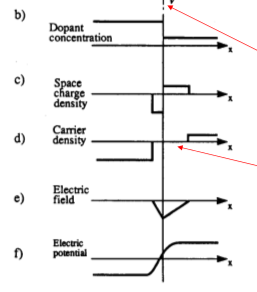
\includegraphics[scale=1]{./Immagini/EquilibrioPN.png}
\caption{Condizione di equilibrio in una giunzione PN}
\label{fig:equilibrioPN}
\end{center}
\end{figure}
Quando viene applicata una differenza di potenziale concorde con quella della regione di svuotamento, la regione si allarga, la corrente di diffusione
diminuisce, mentre quella di generazione (dovuta alla differenza di potenziale alla giunzione) rimane costante.
Come risultato si ottiene un'aumento della corrente di fuga $\propto e^{\frac{qV}{k_B T}}$.
\subsection{Dimensioni della regione di svuotamento}
Supponiamo di aver usato materiali drogati n e p in modo diverso, all'equilibrio la dimensione della regione di svuotamento nelle zone sar\`a asimmetrica.
Se poniamo $N_A$ e $N_D$ la densit\`a lineare di accettori e donori, all'equilibrio vale:
\begin{equation}\label{eq:consCaricaSemicond}
N_A \cdot a = N_D \cdot b
\end{equation}
La densit\`a di carica lineare sar\`a:
\begin{equation*}
\rho (x) = 
\begin{cases}
-e N_A \; \; $se $-a<x<0\\
e N_D \; \; $se $0<x<b
\end{cases}
\end{equation*}
L'equazione di Poisson afferma:
\begin{equation*}
\frac{d^2 \varphi}{dx^2} = \frac{-\rho(x)}{\varepsilon}
\end{equation*}
Integrando una volta la distribuzione di carica si pu\`o ottenere l'opposto del campo elettrico:
\begin{equation*}
-E (x) = 
\begin{cases}
-\frac{e N_A x}{\varepsilon} + c_1 \; \; $se $-a<x<0\\
\frac{e N_D x}{\varepsilon} + c_2 \; \; $se $0<x<b
\end{cases}
\end{equation*}
Imponendo le condizioni al contorno $E(-a)=E(b)=0$ si ottiene:
\begin{equation*}
-E (x) = 
\begin{cases}
-\frac{e N_A (x+a)}{\varepsilon}  \; \; $se $-a<x<0\\
\frac{e N_D (x-b)}{\varepsilon}  \; \; $se $0<x<b
\end{cases}
\end{equation*}
La differenza di potenziale pu\`o essere calcolata tramite:
\begin{equation*}
\Delta V = \left| \int_{-a}^{b} E(x) dx \right| = \frac{e}{2 \varepsilon}(N_A a^2 + N_D b^2)
\end{equation*}
da~\ref{eq:consCaricaSemicond}:
\begin{equation*}
N_D = \frac{N_A \, a}{b}
\end{equation*}
per cui:
\begin{equation*}
\Delta V = \frac{e \, N_A \, a}{2 \varepsilon}(a + b)
\end{equation*}
Se il semiconduttore drogato p debolmente $a \gg b$ e $a \approx d$, con $d$ larghezza della regione di svuotamento, e:
\begin{equation*}
\Delta V = \frac{e \, N_A \, d^2}{2 \varepsilon}
\end{equation*}
da cui si ottiene:
\begin{equation*}
d = \sqrt{\frac{2 \Delta V \, \varepsilon}{e \, N_A}}
\end{equation*}
Essendo:
\begin{equation*}
\rho = \frac{1}{e \mu N}
\end{equation*}
con $N$ numero di portatori di carica maggioritari, si pu\`o anche scrivere:
\begin{equation*}
d = \sqrt{2 \mu \rho \Delta V \, \varepsilon} \approx 0.53 \cdot \sqrt{\Delta V \, \rho}
\end{equation*}
La capacit\`a della giunzione pu\`o essere calcolata come:
\begin{equation*}
C = \frac{\varepsilon}{d} = \sqrt{\frac{e \, N_A \, \varepsilon}{2 \Delta V }}
\end{equation*}
Chiamando $V_b$ il potenziale presente ai capi della regione di svuotamento in assenza di potenziali esterni allora:
\begin{equation*}
\Delta V = V_b + V
\end{equation*}
Aumentando $V$ \`e possibile allargare la regione fino a coprire l'intero semiconduttore; per fare questo, \`e fondamentale unire
un materiale molto drogato con uno poco drogato (altamente intrinseco), in questo modo la regione svuotata risulta priva di portatori
di carica liberi e sensibile alle particelle ionizzanti in quanto all'interno \`e presente un campo in grado di raccogliere le cariche prodotte.
\`E fondamentale un'elevata purezza del materiale, per evitare la presenza di centri di ricombinazione (fermano le lacune) e di intrappolamento (fermano gli elettroni).
\section{Rivelatori al silicio}
\begin{figure}[htbp]
\begin{center}
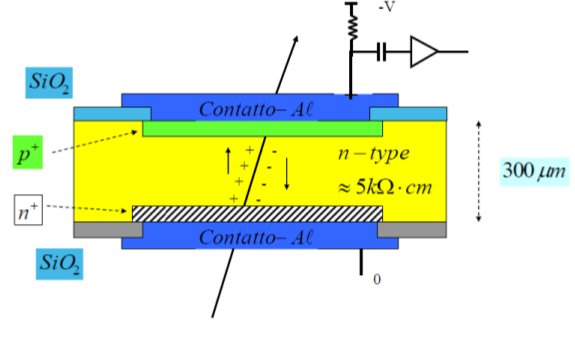
\includegraphics[scale=0.50]{./Immagini/SchemaRivelatoreSilicio.png}
\caption{Schema di un rivelatore al silicio}
\label{fig:schemaRivela49JG8toreSilicio}
\end{center}
\end{figure}
Il silicio \`e molto utilizzato in quanto \`e disponibile a basso costo; il rivelatore \`e formato da una zona fortemente drogata n, che limita
la regione svuotata e funge da contatto ohmico, e da una zona debolmente drogata p, che serve a formare la giunzione.
Dell'ossido di silicio viene formato sulla superfice per passivare il dispositivo ed infine vengono depositati dei sottili contatti di alluminio
(viene scelto l'alluminio perch\`e \`e un materiale con il quale viene bene).
In genere le dimensioni vengono scelte tra i 300 e i 1000 $\mu$m.\\
La carica indotta sugli elettrodi vale:
\begin{equation*}
q(t) \propto \left(1-\text{exp}\left(-\frac{t}{\varepsilon \rho}\right)\right)
\end{equation*}
Il tempo di raccolta del 85\% delle cariche vale:
\begin{equation*}
\tau_e = 2 \rho \varepsilon = 10 \text{ ns}
\end{equation*}
La temperatura operazionale di questi rivelatori pu\`o essere quella ambiente o anche 77 K (azoto liquido) per avere correnti di buio minori;
esistono pi\`u tipi:
\begin{itemize}
\item A barriera superficiale, usati per la spettroscopia $\alpha$ (spessori nel mm)
\item A diffusione, usati per la spettroscopia $\beta$ (spessori nel mm)
\item A deriva di litio, usati per la spettroscopia di X o $\gamma$ a bassa energia (spessori nella decina di mm)
\item Planari passivati, per misure di posizione nella fisica delle alte energie (spessori nel centinaio di $\mu$m)
\end{itemize}
\subsection{Rivelatori a barriera superficiale}
In un rivelatore a barriera superficiale si parte da un silicio non molto drogato n e vi si deposita chimicamente un materiale con un'elevata densit\`a
di trappole per elettroni (difetti).
Questo materiale si comporta come un drogato p fortemente e genera una regione di svuotamento ampia, pur avendo uno strato morto molto sottile; infine sopra questo materiale viene depositato un elettrodo in oro.
Il pregio principale di questa tecnica \`e l'utilizzo di strati morti sottili che assorbono pochissima energia delle $\alpha$ incidenti,
ma proprio per via di questo strato sono sensibili alla luce ambientale (l'energia dei fotoni visibili \`e superiore rispetto a quella del gap), quindi
devono lavorare in condizioni di buio. 
Spesso per la spettroscopia $\alpha$ si lavora in vuoto, di conseguenza la camera a vuoto ha una luminosit\`a trascurabile.\\
La spettroscopia $\alpha$ ottenuta con questi dispositivi ha risoluzioni energetiche nell'ordine dei 10 keV, con un limite statistico a 3 keV.
\subsection{Rivelatori a diffusione}
Un'altra tecnica per fabbricare questi rivelatori consiste nel prendere un wafer drogato debolmente di tipo p ed esponendo una superficie
a vapori di un drogante di tipo n (ad esempio il fosforo): i vapori si diffondono all'interno del wafer (da 0.1 a 2 $\mu$m) portandolo da un
drogaggio di tipo p a uno di tipo n forte.
A questo punto \`e presente uno strato n e uno p, per cui si forma la regione di svuotamento; il problema principale di questa tecnica risiede
nello spessore eccessivo di strato morto, ci\`o rende il dispositivo poco adatto all'impiego nella spettroscopia $\alpha$, ma buono per l'impiego
in spettroscopia $\beta$.\\
Lo strato morto del dispositivo risulta comunque valutabile studiando l'energia persa in funzione dell'angolo di incidenza.
\section{Rivelatori HPGe}
La bassa energia di gap del germanio rende inadatto l'uso a temperatura ambiente, tuttavia a basse temperature (77 K) esso risulta utilizzabile
per effettuare spettroscopia.
Grazie all'elevata purezza raggiungibile con i cristalli di germanio \`e possibile realizzare rivelatori grandi decine di cm$^3$, inoltre
lo $Z=32$ del Ge per la spettroscopia $\gamma$ ad alta risoluzione.
Vengono ottenute grandi regioni di svuotamento attraverso una giunzione p-i-n.
\begin{figure}[htbp]
\begin{center}
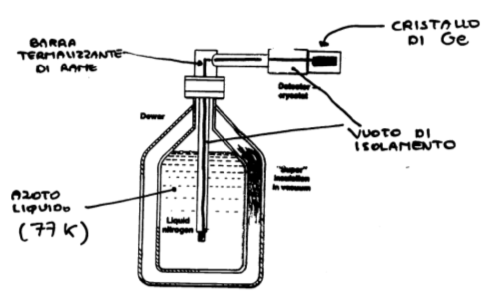
\includegraphics[scale=1]{./Immagini/SchemaHPGe.png}
\caption{Schema di un HPGe, il PRE in questi dispositivi sta nella camera a vuoto, per ridurre al minimo la capacit\`a dei cavi}
\label{fig:schemaHPGe}
\end{center}
\end{figure}